\section{最急降下法と勾配降下法}

\begin{frame}[t,fragile]{最急降下法(steepest descent)}
  \begin{itemize}
    \setlength{\itemsep}{1em}
  \item 関数の微分の情報を使う
  \item 現在の点$\bf x$における勾配を計算
    \[
    -\nabla f|_i = -\frac{\partial f}{\partial x_i}
    \]
  \item 坂を下る方向にそって、一次元最適化
  \item 動いた先の勾配の方向でさらに最適化を繰り返す
  \item 関数値は単調減少 $\Rightarrow$ 極小値に収束
  \end{itemize}
\end{frame}

\begin{frame}[t,fragile]{勾配降下法(gradient descent)}
  \begin{itemize}
    \setlength{\itemsep}{1em}
  \item 勾配方向に一次元最適化を行うかわりに、あらかじめ決めた一定量($\epsilon$)だけ坂を下る
    \[
    x_{n+1} = x_n - \epsilon \, \nabla f
    \]
  \item あらかじめ最適な$\epsilon$を知るのは困難
  \item 機械学習の分野では、(なぜか) $\epsilon=0.1$が良いとされている
  \item この方法を「最急降下法」、一次元最適化を行う勾配法を「最適降下法(optimum descent)」と呼ぶ場合も
  % \item c.f.) 確率的勾配降下法(stochastic gradient descent)
  \end{itemize}
\end{frame}

\begin{frame}[t,fragile]{制約条件付きの場合}
  \begin{itemize}
    % \setlength{\itemsep}{1em}
  \item 目的関数: $f(x)$
  \item 制約条件:
    \begin{itemize}
    \item $g_i(x) = 0$ \ ($i=1,\cdots,m$) \ (等式制約条件)
    \item $h_j(x) \ge 0$ \ ($j=1,\cdots,n$) \ (不等式制約条件)
    \end{itemize}
  \item 等式制約条件の付いている場合: Lagrangeの未定乗数法
    \[
    L(x,\lambda_1,\cdots,\lambda_m)=f(x)+\sum_i \lambda_i g_i(x)
    \]
    を考え、$x,\lambda_1,\cdots,\lambda_m$の微分が零となる点を探す
  \item 不等式制約条件の付いている場合: c.f. 線形計画法, ペナルティ関数法
  \end{itemize}
\end{frame}

\begin{frame}[t,fragile]{細長い谷の場合}
  \vspace*{1em}
  \hspace*{1em}\resizebox{1\textwidth}{!}{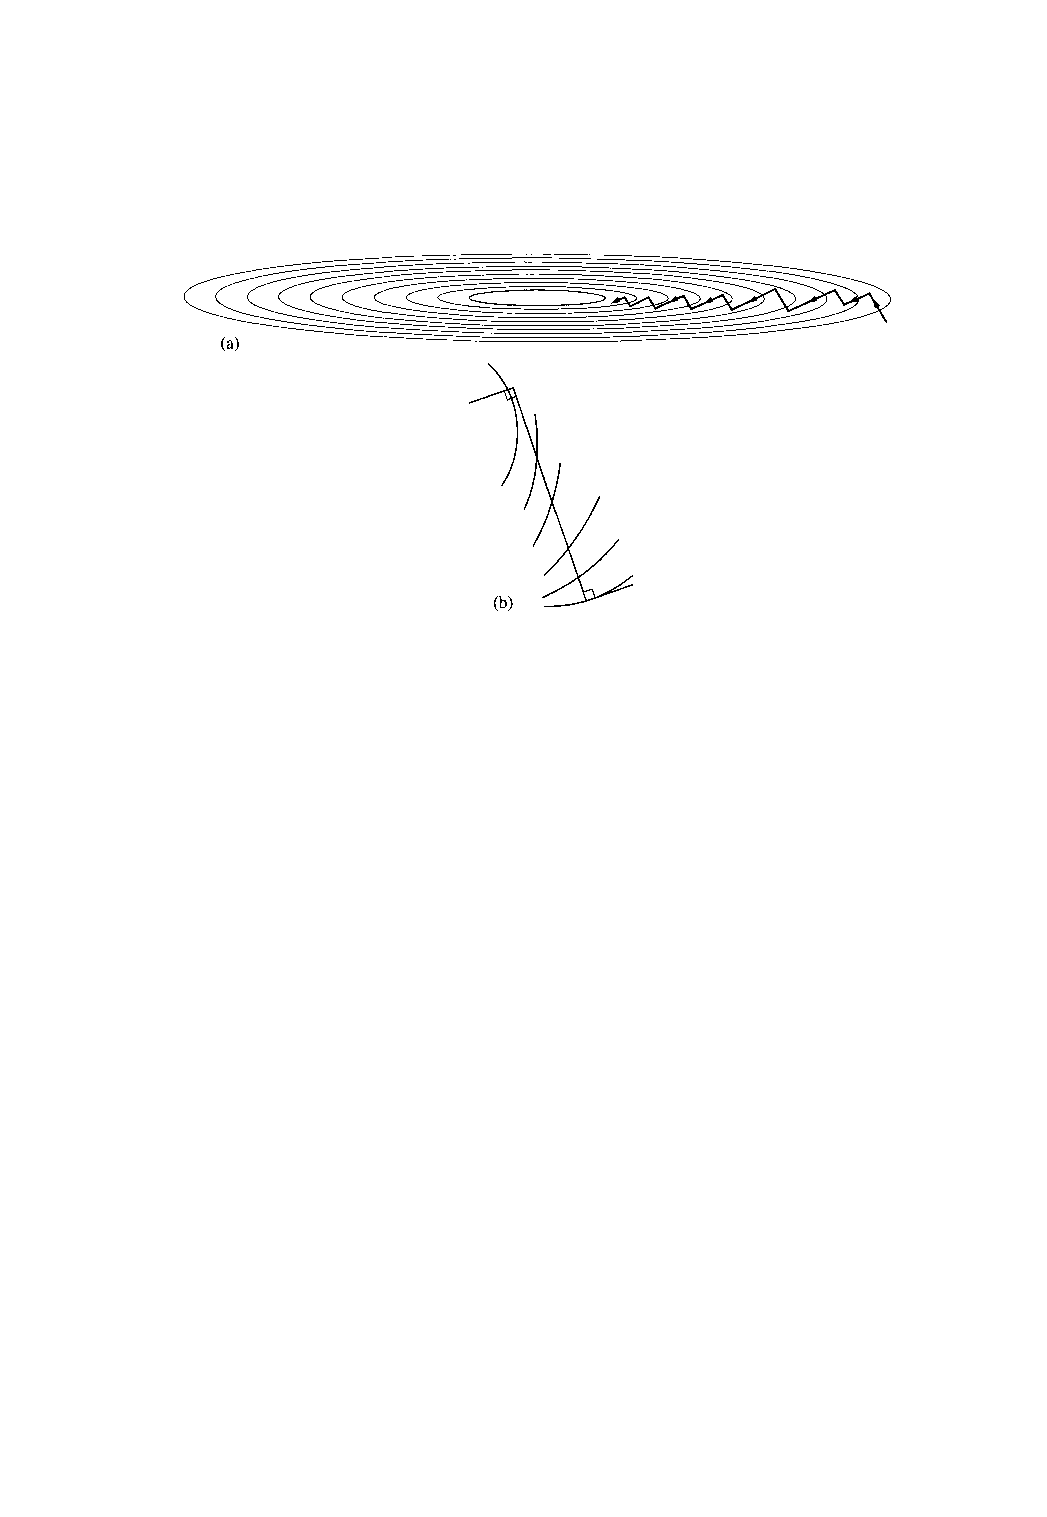
\includegraphics{image/steepest-descent.pdf}}

  \vspace*{-2em}
  \hspace*{20em}{\footnotesize(Press et al 1988)}
\end{frame}
